\section{Architettura generale} \label{archGen}

    \begin{figure}[htbp]
        \centering
        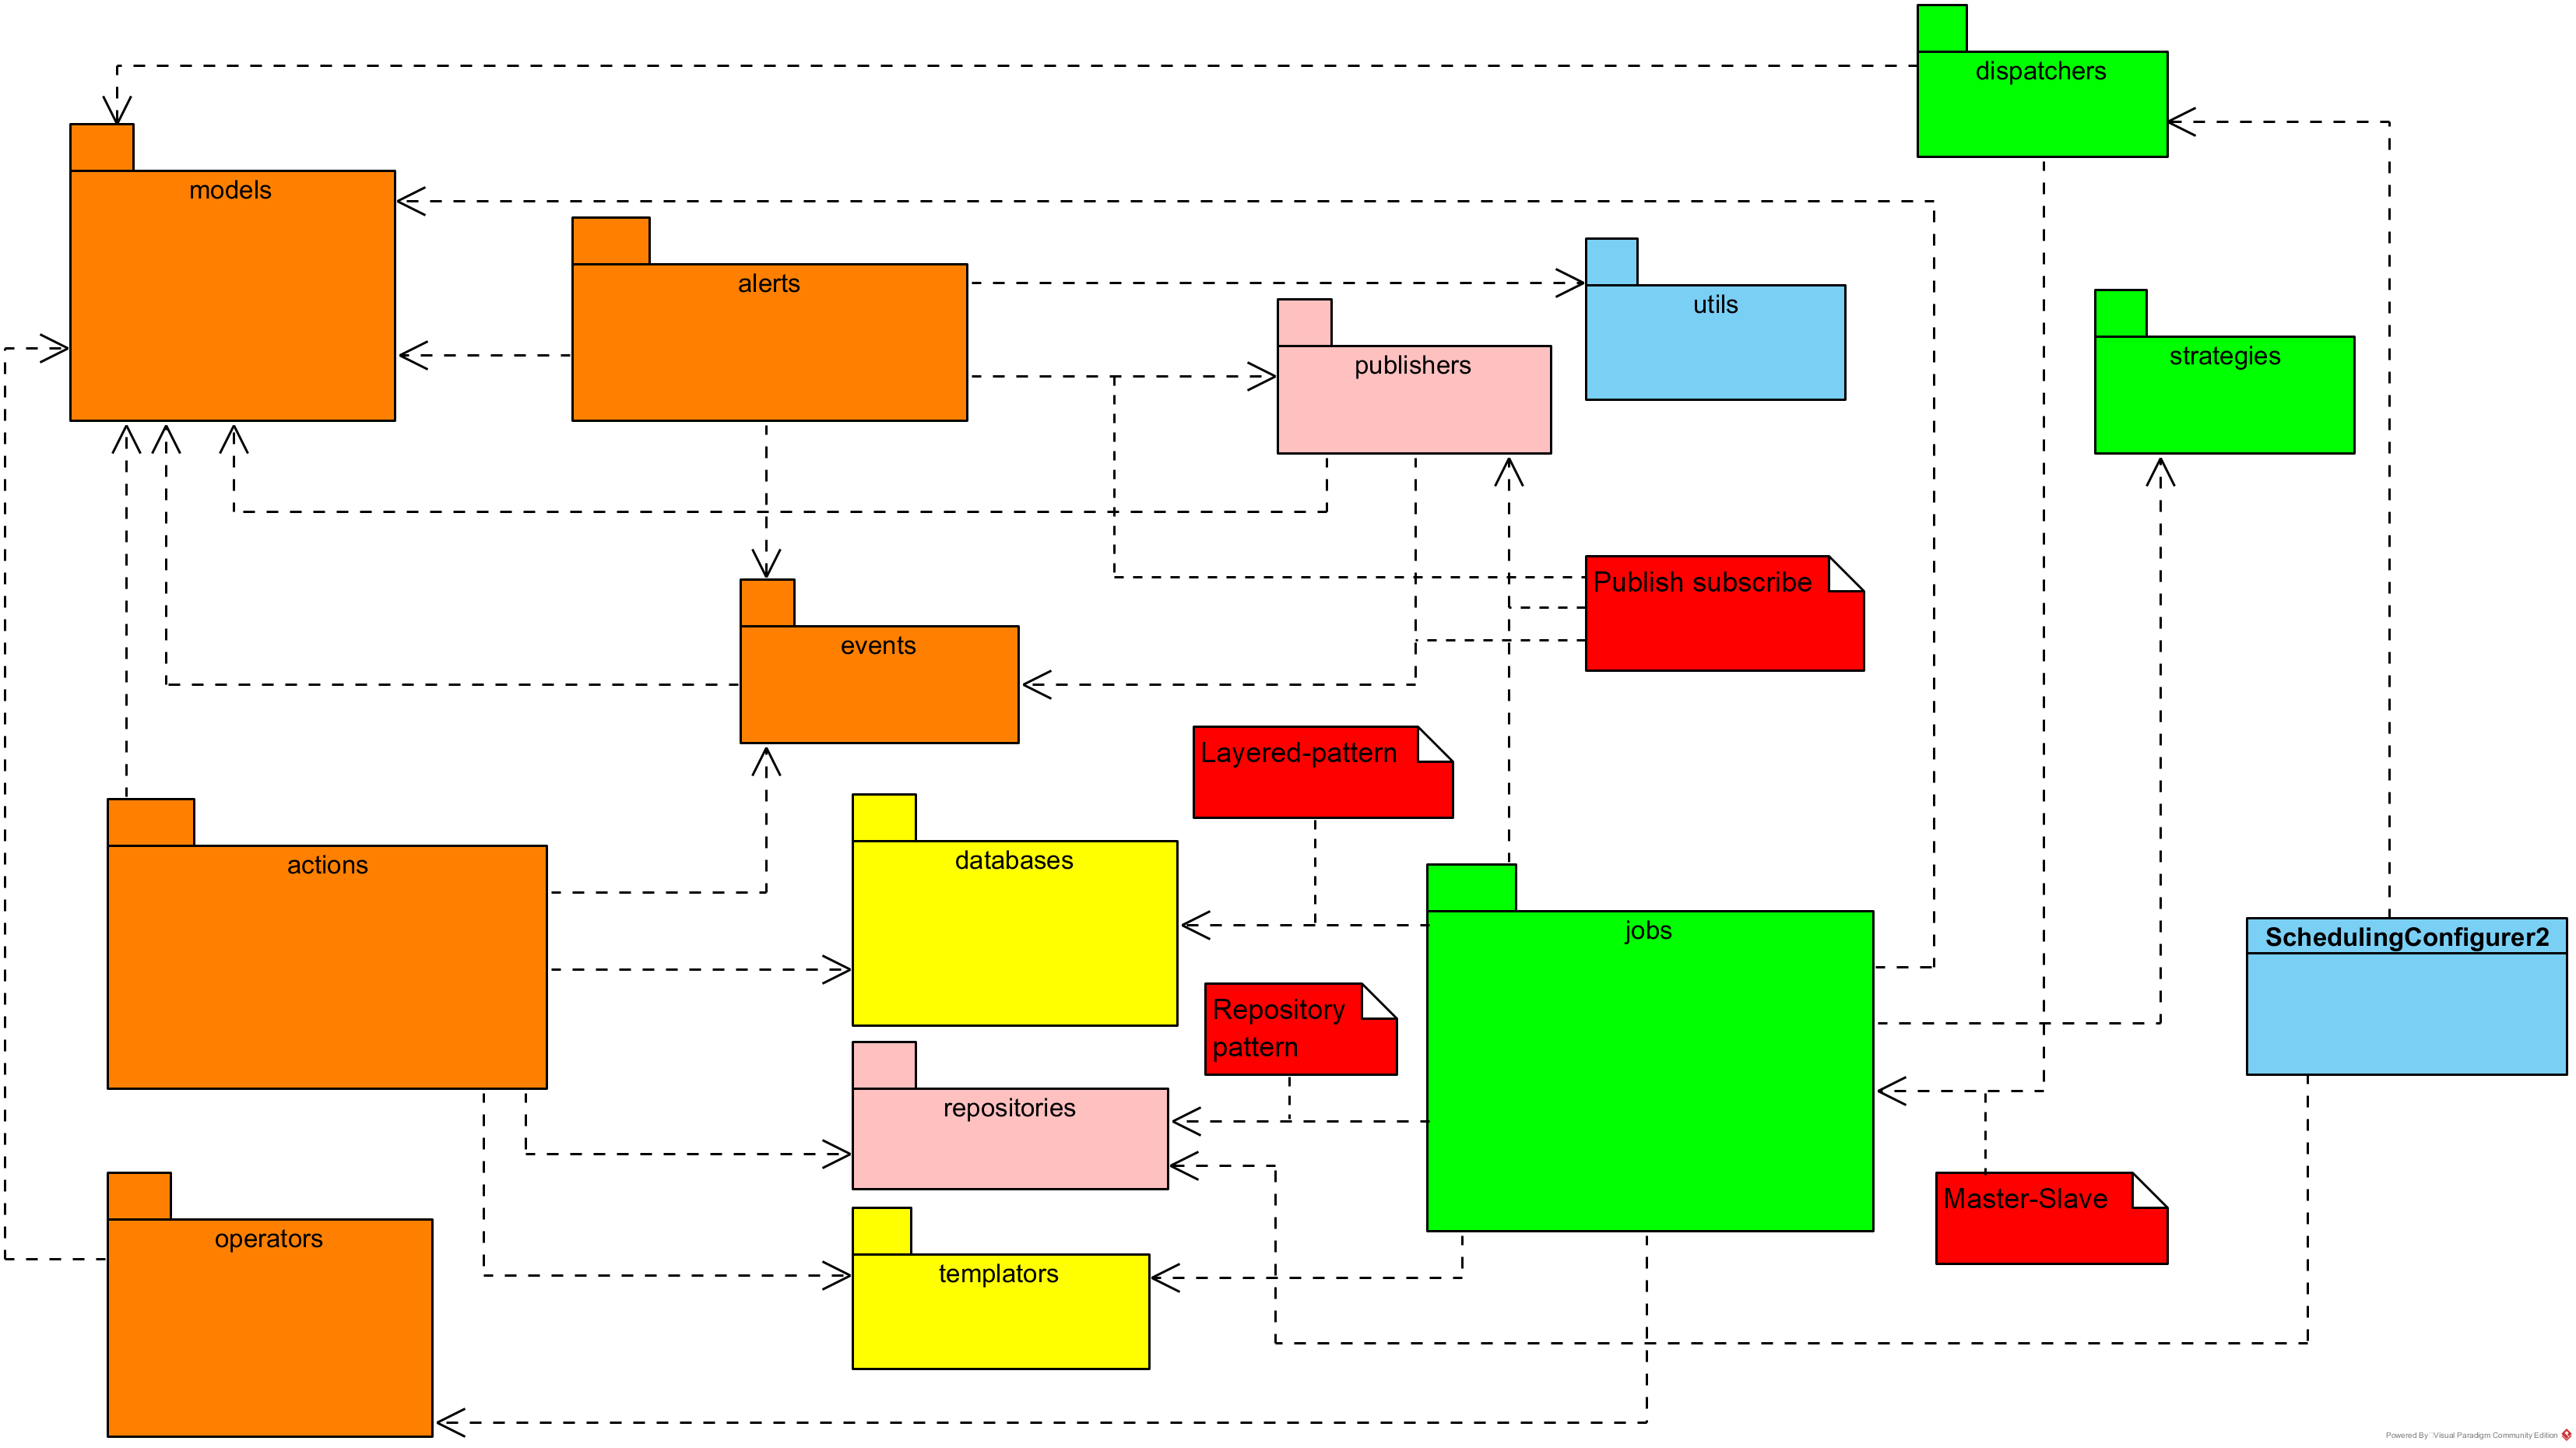
\includegraphics[width=\textwidth]{./img/ArchitetturaGenerale/generalArchitecture.png}
        \caption[Architettura generale della applicazione]{Architettura generale dell'applicazione}
    \end{figure}
    
    L'immagine raffigura il diagramma dei package che descrive l'architettura generale dell'applicazione.
    L'applicativo è composto dalle seguenti parti:

    \begin{itemize}
    	\item \textbf{Scheduler Configurer}: classe che si occupa di configurare lo scheduler di Spring. Si occupa della
    	creazione dei dispatchers utili al funzionamento dell'applicazione;
    	\item \textbf{actions}: package che contiene tutte le classi che rappresentano azioni di rimedio. Le azioni di
    	rimedio vengono eseguite nel caso in cui si verifichi un alert;
    	\item \textbf{alerts}: package che contiene le classi che descrivono lo scatenarsi di un evento in cui è necessario
    	eseguire un'azione di rimedio;
    	\item \textbf{databases}: package che contiene classi necessarie alla raccolta di dati utili durante l'esecuzione;
    	\item \textbf{dispatchers}: package che contiene le classi che permettono la creazione di dispachers per la
    	richiesta di generazione di \glossaryItem{metriche} e baseline;
    	\item \textbf{events}: package che contiene le classi che rappresentano il manifestarsi di un evento;
    	\item \textbf{jobs}: package che contiene le classi che rappresentano le operazioni che può svolgere l'applicazione;
    	\item \textbf{models}: package che contiene le classi che rappresentano tutte le configurazioni per le componenti
    	dell'applicazione;
    	\item \textbf{operators}: package che raccoglie tutti gli operatori coinvolti nei diversi calcoli presenti
    	nell'applicazione;
    	\item \textbf{publishers}: package che contiene le classi che si occupano di generare notifiche dell'avvenimento
    	di un evento (metrica generata, alert generato);
    	\item \textbf{repositories}:  package che contiene le classi necessarie per prelevare le configurazioni degli oggetti
    	da Elasticsearch;
    	\item \textbf{strategies}: package che contiene le classi che descrivono le strategie con cui si recuperano le baseline;
    	\item \textbf{templators}: package che contiene le classi utili a creare date e operatori;
    	\item \textbf{utils}: package che contiene classi di utilità.
    \end{itemize}
